\documentclass[twoside]{book}

% Packages required by doxygen
\usepackage{fixltx2e}
\usepackage{calc}
\usepackage{doxygen}
\usepackage[export]{adjustbox} % also loads graphicx
\usepackage{graphicx}
\usepackage[utf8]{inputenc}
\usepackage{makeidx}
\usepackage{multicol}
\usepackage{multirow}
\PassOptionsToPackage{warn}{textcomp}
\usepackage{textcomp}
\usepackage[nointegrals]{wasysym}
\usepackage[table]{xcolor}

% Font selection
\usepackage[T1]{fontenc}
\usepackage[scaled=.90]{helvet}
\usepackage{courier}
\usepackage{amssymb}
\usepackage{sectsty}
\renewcommand{\familydefault}{\sfdefault}
\allsectionsfont{%
  \fontseries{bc}\selectfont%
  \color{darkgray}%
}
\renewcommand{\DoxyLabelFont}{%
  \fontseries{bc}\selectfont%
  \color{darkgray}%
}
\newcommand{\+}{\discretionary{\mbox{\scriptsize$\hookleftarrow$}}{}{}}

% Page & text layout
\usepackage{geometry}
\geometry{%
  a4paper,%
  top=2.5cm,%
  bottom=2.5cm,%
  left=2.5cm,%
  right=2.5cm%
}
\tolerance=750
\hfuzz=15pt
\hbadness=750
\setlength{\emergencystretch}{15pt}
\setlength{\parindent}{0cm}
\setlength{\parskip}{3ex plus 2ex minus 2ex}
\makeatletter
\renewcommand{\paragraph}{%
  \@startsection{paragraph}{4}{0ex}{-1.0ex}{1.0ex}{%
    \normalfont\normalsize\bfseries\SS@parafont%
  }%
}
\renewcommand{\subparagraph}{%
  \@startsection{subparagraph}{5}{0ex}{-1.0ex}{1.0ex}{%
    \normalfont\normalsize\bfseries\SS@subparafont%
  }%
}
\makeatother

% Headers & footers
\usepackage{fancyhdr}
\pagestyle{fancyplain}
\fancyhead[LE]{\fancyplain{}{\bfseries\thepage}}
\fancyhead[CE]{\fancyplain{}{}}
\fancyhead[RE]{\fancyplain{}{\bfseries\leftmark}}
\fancyhead[LO]{\fancyplain{}{\bfseries\rightmark}}
\fancyhead[CO]{\fancyplain{}{}}
\fancyhead[RO]{\fancyplain{}{\bfseries\thepage}}
\fancyfoot[LE]{\fancyplain{}{}}
\fancyfoot[CE]{\fancyplain{}{}}
\fancyfoot[RE]{\fancyplain{}{\bfseries\scriptsize Generated by Doxygen }}
\fancyfoot[LO]{\fancyplain{}{\bfseries\scriptsize Generated by Doxygen }}
\fancyfoot[CO]{\fancyplain{}{}}
\fancyfoot[RO]{\fancyplain{}{}}
\renewcommand{\footrulewidth}{0.4pt}
\renewcommand{\chaptermark}[1]{%
  \markboth{#1}{}%
}
\renewcommand{\sectionmark}[1]{%
  \markright{\thesection\ #1}%
}

% Indices & bibliography
\usepackage{natbib}
\usepackage[titles]{tocloft}
\setcounter{tocdepth}{3}
\setcounter{secnumdepth}{5}
\makeindex

% Hyperlinks (required, but should be loaded last)
\usepackage{ifpdf}
\ifpdf
  \usepackage[pdftex,pagebackref=true]{hyperref}
\else
  \usepackage[ps2pdf,pagebackref=true]{hyperref}
\fi
\hypersetup{%
  colorlinks=true,%
  linkcolor=blue,%
  citecolor=blue,%
  unicode%
}

% Custom commands
\newcommand{\clearemptydoublepage}{%
  \newpage{\pagestyle{empty}\cleardoublepage}%
}

\usepackage{caption}
\captionsetup{labelsep=space,justification=centering,font={bf},singlelinecheck=off,skip=4pt,position=top}

%===== C O N T E N T S =====

\begin{document}

% Titlepage & ToC
\hypersetup{pageanchor=false,
             bookmarksnumbered=true,
             pdfencoding=unicode
            }
\pagenumbering{alph}
\begin{titlepage}
\vspace*{7cm}
\begin{center}%
{\Large Menu }\\
\vspace*{1cm}
{\large Generated by Doxygen 1.8.13}\\
\end{center}
\end{titlepage}
\clearemptydoublepage
\pagenumbering{roman}
\tableofcontents
\clearemptydoublepage
\pagenumbering{arabic}
\hypersetup{pageanchor=true}

%--- Begin generated contents ---
\chapter{Class Index}
\section{Class List}
Here are the classes, structs, unions and interfaces with brief descriptions\+:\begin{DoxyCompactList}
\item\contentsline{section}{\hyperlink{class_menu}{Menu} \\*The \hyperlink{class_menu}{Menu} class }{\pageref{class_menu}}{}
\end{DoxyCompactList}

\chapter{File Index}
\section{File List}
Here is a list of all documented files with brief descriptions\+:\begin{DoxyCompactList}
\item\contentsline{section}{\hyperlink{menu_8cpp}{menu.\+cpp} \\*Implémentation de la classe \hyperlink{class_menu}{Menu} }{\pageref{menu_8cpp}}{}
\item\contentsline{section}{{\bfseries menu.\+h} }{\pageref{menu_8h}}{}
\end{DoxyCompactList}

\chapter{Class Documentation}
\hypertarget{class_menu}{}\section{Menu Class Reference}
\label{class_menu}\index{Menu@{Menu}}


The \hyperlink{class_menu}{Menu} class.  




{\ttfamily \#include $<$menu.\+h$>$}

\subsection*{Public Member Functions}
\begin{DoxyCompactItemize}
\item 
\hyperlink{class_menu_a2733b73d7c4dff4b1db19afd45f255b9}{Menu} (const string \&\+\_\+nom)
\begin{DoxyCompactList}\small\item\em \hyperlink{class_menu}{Menu}. \end{DoxyCompactList}\item 
\hyperlink{class_menu_a831387f51358cfb88cd018e1777bc980}{$\sim$\+Menu} ()
\begin{DoxyCompactList}\small\item\em \hyperlink{class_menu_a831387f51358cfb88cd018e1777bc980}{Menu\+::$\sim$\+Menu}. \end{DoxyCompactList}\item 
int \hyperlink{class_menu_a079e0c6a24248a07993b48b310ba65ce}{Afficher} ()
\begin{DoxyCompactList}\small\item\em Afficher. \end{DoxyCompactList}\end{DoxyCompactItemize}
\subsection*{Static Public Member Functions}
\begin{DoxyCompactItemize}
\item 
static void \hyperlink{class_menu_a6ddcaabf2fedb30f5136f3be655d60ce}{Attendre\+Appui\+Touche} ()
\begin{DoxyCompactList}\small\item\em Attendre\+Appui\+Touche. \end{DoxyCompactList}\end{DoxyCompactItemize}


\subsection{Detailed Description}
The \hyperlink{class_menu}{Menu} class. 

\subsection{Constructor \& Destructor Documentation}
\mbox{\Hypertarget{class_menu_a2733b73d7c4dff4b1db19afd45f255b9}\label{class_menu_a2733b73d7c4dff4b1db19afd45f255b9}} 
\index{Menu@{Menu}!Menu@{Menu}}
\index{Menu@{Menu}!Menu@{Menu}}
\subsubsection{\texorpdfstring{Menu()}{Menu()}}
{\footnotesize\ttfamily Menu\+::\+Menu (\begin{DoxyParamCaption}\item[{const string \&}]{\+\_\+nom }\end{DoxyParamCaption})}



\hyperlink{class_menu}{Menu}. 

\hyperlink{class_menu_a2733b73d7c4dff4b1db19afd45f255b9}{Menu\+::\+Menu}.


\begin{DoxyParams}{Parameters}
{\em \+\_\+nom} & \\
\hline
{\em \+\_\+nom} & \\
\hline
\end{DoxyParams}
Constructeur de la classe menu calcul le nombre d\textquotesingle{}options pour allouer de la place \mbox{\Hypertarget{class_menu_a831387f51358cfb88cd018e1777bc980}\label{class_menu_a831387f51358cfb88cd018e1777bc980}} 
\index{Menu@{Menu}!````~Menu@{$\sim$\+Menu}}
\index{````~Menu@{$\sim$\+Menu}!Menu@{Menu}}
\subsubsection{\texorpdfstring{$\sim$\+Menu()}{~Menu()}}
{\footnotesize\ttfamily Menu\+::$\sim$\+Menu (\begin{DoxyParamCaption}{ }\end{DoxyParamCaption})}



\hyperlink{class_menu_a831387f51358cfb88cd018e1777bc980}{Menu\+::$\sim$\+Menu}. 

deconstructeur de la clase menu 

\subsection{Member Function Documentation}
\mbox{\Hypertarget{class_menu_a079e0c6a24248a07993b48b310ba65ce}\label{class_menu_a079e0c6a24248a07993b48b310ba65ce}} 
\index{Menu@{Menu}!Afficher@{Afficher}}
\index{Afficher@{Afficher}!Menu@{Menu}}
\subsubsection{\texorpdfstring{Afficher()}{Afficher()}}
{\footnotesize\ttfamily int Menu\+::\+Afficher (\begin{DoxyParamCaption}{ }\end{DoxyParamCaption})}



Afficher. 

\hyperlink{class_menu_a079e0c6a24248a07993b48b310ba65ce}{Menu\+::\+Afficher}.

\begin{DoxyReturn}{Returns}

\end{DoxyReturn}
Afficher le menu dans une fenetre \begin{DoxyReturn}{Returns}

\end{DoxyReturn}
\mbox{\Hypertarget{class_menu_a6ddcaabf2fedb30f5136f3be655d60ce}\label{class_menu_a6ddcaabf2fedb30f5136f3be655d60ce}} 
\index{Menu@{Menu}!Attendre\+Appui\+Touche@{Attendre\+Appui\+Touche}}
\index{Attendre\+Appui\+Touche@{Attendre\+Appui\+Touche}!Menu@{Menu}}
\subsubsection{\texorpdfstring{Attendre\+Appui\+Touche()}{AttendreAppuiTouche()}}
{\footnotesize\ttfamily void Menu\+::\+Attendre\+Appui\+Touche (\begin{DoxyParamCaption}{ }\end{DoxyParamCaption})\hspace{0.3cm}{\ttfamily [static]}}



Attendre\+Appui\+Touche. 

\hyperlink{class_menu_a6ddcaabf2fedb30f5136f3be655d60ce}{Menu\+::\+Attendre\+Appui\+Touche}.

fonction qui attend que l\textquotesingle{}utilisateur appuie sur une touche pour continuer 

The documentation for this class was generated from the following files\+:\begin{DoxyCompactItemize}
\item 
menu.\+h\item 
\hyperlink{menu_8cpp}{menu.\+cpp}\end{DoxyCompactItemize}

\chapter{File Documentation}
\hypertarget{menu_8cpp}{}\section{menu.\+cpp File Reference}
\label{menu_8cpp}\index{menu.\+cpp@{menu.\+cpp}}


Implémentation de la classe \hyperlink{class_menu}{Menu}.  


{\ttfamily \#include \char`\"{}menu.\+h\char`\"{}}\newline
Include dependency graph for menu.\+cpp\+:
\nopagebreak
\begin{figure}[H]
\begin{center}
\leavevmode
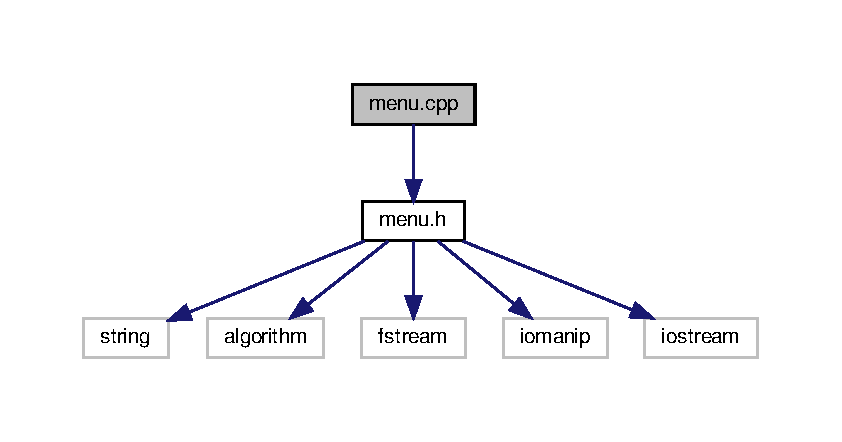
\includegraphics[width=350pt]{menu_8cpp__incl}
\end{center}
\end{figure}


\subsection{Detailed Description}
Implémentation de la classe \hyperlink{class_menu}{Menu}. 

\begin{DoxyVersion}{Version}
1.\+1 
\end{DoxyVersion}
\begin{DoxyAuthor}{Author}
Jonathan R\+I\+B\+E\+I\+RO 
\end{DoxyAuthor}
\begin{DoxyDate}{Date}
13 sept 2019 
\end{DoxyDate}

%--- End generated contents ---

% Index
\backmatter
\newpage
\phantomsection
\clearemptydoublepage
\addcontentsline{toc}{chapter}{Index}
\printindex

\end{document}
